The best way to show the clustering results is plotting the trajectory with different colours in relation to the cluster which it belongs. In addiction, for clustering algorithms, I used a method of interpretation and validation of consistency within clusters of data, called \textit{Silhouette}. 

\textit{Silhouette} clustering validation technique measures how similar an object is to its own cluster compared to other clusters. The silhouette ranges from -1 to +1, where a high value indicates that the object is well matched to its own cluster and poorly matched to neighbouring clusters.

The results of heuristic analysis are the following: 
\begin{itemize}
	\item \textit{timedelta heuristic}: in figure \ref{fig:timedelta-result} you can see some rentals with their positions divided in subgroups of trajectories. That sub trajectories are built considering only the time gaps between the positions, no latitude or longitude has been used to produce this result. This result shows how the time sequences could be really useful to produce a good trajectory partition.
	
	\begin{figure}[bt]
		\centering
		\includegraphics[width=\columnwidth]{timedelta-result}
		\caption{Timedelta heuristic line plot in details}
		\label{fig:timedelta-result}
	\end{figure}
	
	\item \textit{spreddelta heuristic}: in figure \ref{fig:spreaddelta-result} you can see how the trajectories are clusterized in 3 main groups: wide area trajectories (green), medium area trajectories (blue) and small area trajectories (red).
	
	\begin{figure}[bt]
		\centering
		\includegraphics[width=\columnwidth]{spreaddelta-result}
		\caption{Spreaddelta heuristic line plot}
		\label{fig:spreaddelta-result}
	\end{figure}
	
	\item \textit{edgedelta heuristic}: in figure \ref{fig:edgedelta-result} you can see how the trajectories are clusterized in relation to the start and end positions of each trajectory generated by \textit{timedelta heuristic}. 
	
	\begin{figure}[bt]
		\centering
		\includegraphics[width=\columnwidth]{edgedelta-result}
		\caption{Edgedelta heuristic line plot}
		\label{fig:edgedelta-result}
	\end{figure}
	
\end{itemize}

For clustering algorithms, in addition to graph analysis, I also use the \textit{Silhouette} validation. To evaluate the number of clusters for the algorithms that need it as parameter, I executed \textit{K-Means} for a number of cluster in a range from 1 to 30 and I calculated for each cluster number the \textit{WCSS error}. Then I plot the \textit{WCSS} graph and I used \textit{Elbow method} to choose the best value to use. As result of \textit{WCSS} graph, I chose to set 5 clusters. 

\begin{figure}[bt]
	\centering
	\includegraphics[width=\columnwidth]{wcss}
	\caption{Within Cluster Sum of Squares (WCSS) graph for Elbow method in range 1 to 30 with K-Means}
	\label{fig:wcss}
\end{figure}

All clustering techniques were performed on each city individually, in order to facilitate the algorithms. The results of clustering techniques are the following: 

\begin{itemize}
	\item \textit{Gaussian Mixture}: performs bad result \ref{fig:gaussian-mixture-line} and the silhouette validation confirms it (silhouette -0.02).
	
	\item \textit{Mean Shift}: obtains the best result in terms of silhouette validation (silhouette 0.40). The number of cluster generated is only 3 because \textit{Mean Shift}, at the end of algorithm, performs a pruning operation of similar centres, taking only the more significant. In general, for trajectory clustering, I would like to obtain more clusters, but this is also an alert that the number of clusters can't be really higher. 
	
	\item \textit{Full Hierarchical Agglomerative}: worst in silhouette validation term (0.16), but the main issue of this technique is a huge memory cost. The dedrogram of this hierarchical algorithm is shown in the this figure \ref{fig:full-agglomerative-dendrogram}. 
	
	\begin{figure}[bt]
		\centering
		\includegraphics[width=\columnwidth]{full-agglomerative-dendrogram}
		\caption{Full Hierarchical Agglomerative dendrogram up to level 5 of merge}
		\label{fig:full-agglomerative-dendrogram}
	\end{figure}
	
	\item \textit{Ward Hierarchical Agglomerative}: performs well because it tries to group the centre of the city. It is really similar to \textit{K-Means}, but it is not as accurate as \textit{K-Means} (silhouette 0.28).

	\item \textit{K-Means}: it is the simplest algorithm but maybe the one that produces the best results. Even if it uses a distance metric to calculate the clusters, it performs very well not only in terms of plot representation, but also in silhouette value. In addition, it is really fast and cheap in memory. The main problem of this clustering result is the mixture of clusters in the city centre, that creates uncertainty.
	
	\begin{figure}[bt]
		\centering
		\includegraphics[width=\columnwidth]{k-means-plot}
		\caption{K-Means line plot with silhouette 0.352}
		\label{fig:k-means-line}
	\end{figure}
\end{itemize}

The deep clustering techniques have been tested with a learning rate of $10^{-3}$ and from 10 to 30 epochs, but do not produce very interesting results as shown in the figure \ref{fig:dl-clustering}. All 3 autoencoder models have been tested with the use of the moving behavior extration algorithm and produce similar results.

\begin{figure}[bt]
	\centering
	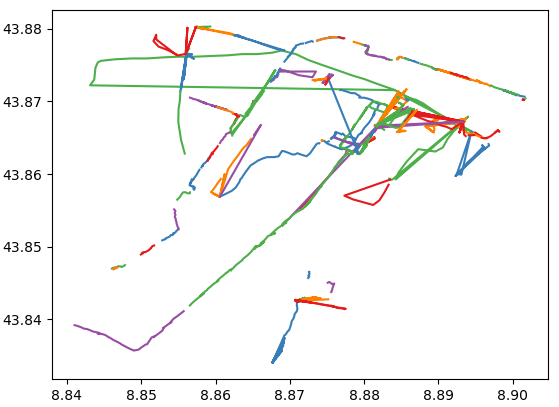
\includegraphics[width=\columnwidth]{dl-clustering}
	\caption{Deep Learning Clustering result with Autoencoder}
	\label{fig:dl-clustering}
\end{figure}